%\documentclass[11pt]{beamer}
\usepackage[ngerman]{babel}
\usepackage[utf8]{inputenc}
\usepackage{amsmath}
\usepackage{amssymb}
\usepackage{listings} 
\usepackage{stmaryrd}
\lstset{language=Python, tabsize=4, showstringspaces=false,basicstyle=\footnotesize,mathescape=true} 
\lstset{literate=%
  {Ö}{{\"O}}1
  {Ä}{{\"A}}1
  {Ü}{{\"U}}1
  {ß}{{\ss}}1
  {ü}{{\"u}}1
  {ä}{{\"a}}1
  {ö}{{\"o}}1
}
\usepackage{mathtools}
\usepackage{ulem}
\usepackage{tikz}

\usetheme{Boadilla}
\mode<presentation>{
\useoutertheme[subsection=false]{miniframes}
\useinnertheme{rectangles}
%\usecolortheme{crane}
}
\parskip 10pt
\newcommand{\ggT}{\operatorname{ggT}}
\newcommand{\Mod}[3]{#1\equiv#2\text{ mod }#3}
\newcommand{\tmod}{\text{ mod }}


\begin{document}
\title{Vertiefungskurs Mathematik}   
\author{Kryptographie} 
\date{}
\frame{\titlepage} 

%---
\begin{frame}[fragile]

Kryptographie ist die Wissenschaft der Verschlüsselung von Informationen. \pause

\textbf{Diffie-Hellman Schlüsselaustausch} \pause

Alice und Bob vereinbaren eine Primzahl $p$ und eine Generatorzahl $g \in \{1,2,...p-1\}$, am besten eine Primitivwurzel in 
$\mathbb{Z}_p$. \pause Alice wählt geheim eine Zahl $a$ aus, Bob geheim eine Zahl $b$ mit $a,b \in \{1,2,...p-1\}$. \pause
Alice berechnet $A = g^a \tmod p$,  $B = g^b \tmod p$. \pause Dann tauschen beide $A$ und $B$ aus. \pause Das bedeutet, 
$p,g,A,B$ sind öffentlich bekannt, $a$ kennt nur Alice, $b$ nur Bob. \pause

Beide können nun den gemeinsamen Schlüssel $K$ berechnen: \\
Alice: $B^a \equiv (g^b)^a \equiv g^{ba} \equiv K \tmod p$ \\
Bob: $A^b \equiv (g^a)^b \equiv g^{ab} \equiv K \tmod p$ 

\end{frame}

 %---
\begin{frame}[fragile]

Beispiel: $p=13, g=2$ \\ \pause
Alice: $a=5, \quad \pause A \equiv 2^5 \equiv 6 \tmod 13$ \\
Bob: $b=8, \quad \pause B \equiv 2^8 \equiv 9 \tmod 13$ \pause

Schlüssel berechnen: \\ \pause
Alice: $B^a \equiv 9^5 \equiv 3 \tmod 13 \Rightarrow K = 3$ \\ \pause
Bob: $A^b \equiv 6^8 \equiv 3 \tmod 13 \Rightarrow K = 3$ \pause

\footnotesize
Nebenrechnungen (mod 13): \\
\begin{tabular}{l l l}
$2^1 \equiv 2$    &  \quad &  $6^1 \equiv 6$  \\
$2^2 \equiv 4$    &    &  $6^2 \equiv 36 \equiv -3$ \\
$2^4 \equiv 3$    &   &  $6^4 \equiv 9 \equiv -4$ \\
& & $6^8 \equiv 16 \equiv 3$  \\
$9^1 \equiv -4$ \\
$9^2 \equiv 16 \equiv 3$\\
$9^4 \equiv -4 $
\end{tabular}
\end{frame}


 %---
\begin{frame}[fragile]

\textbf{Angriff auf Diffie-Hellman} \pause

Eve versucht aus den öffentlich bekannten Zahlen $p,g,A,B$ den Schlüssel $K$ zu berechnen. \pause
Eve weiß: $2^a \equiv 6 \tmod 13$ und $2^b \equiv 9 \tmod 13$. \pause

\begin{tabular}{ll}
\begin{minipage}[b]{8cm}
Die Beschaffung des Exponenten $a$ oder $b$ heißt `Berechnung des diskreten Logarithmus'. \pause Bei kleinen
Zahlen ist dies durch Ausprobieren möglich.  $g$ sollte Primitivwurzel sein, damit Angreifer möglichst viel ausprobieren muss.  
\end{minipage} &
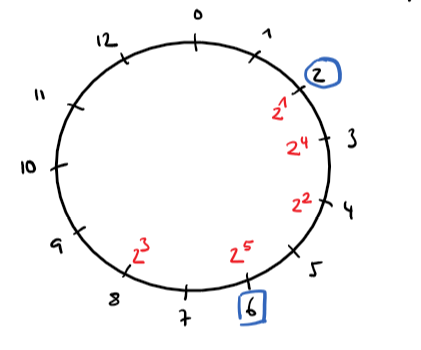
\includegraphics[height=3.5cm]{bild2.png}
\end{tabular} \pause

In der Praxis ist $p$ eine Primzahl mit ca. 300 Stellen (eine Zahl größer als die Anzahl Atome im Weltall). Es 
ist kein effektives Verfahren zur Berechnung des diskreten Logarithmus bekannt.
\end{frame}

 %---
\begin{frame}[fragile]

\textbf{Unterschied Logarithmus in $\mathbb{Z}_p$ und Logarithmus in $\mathbb{R}$} \pause

Beim Rechnen in $\mathbb{R}$ kann man den Wert des Exponenten abschätzen. \pause

Beispiel: Gesucht ist $a \in \mathbb{R}$ mit $2^a = 12$. \pause Wegen $2^3 = 8$ und $2^4 = 16$ folgt: $3 < a < 4$. \pause
Diese Folgerung ist im diskreten Fall nicht möglich. \pause  Die Potenzen der Generatorzahl springen wie zufällig in dem Restklassenring herum.
\end{frame}


 %---
\begin{frame}[fragile]

\textbf{Man-in-the-middle-Angriff auf Diffie-Hellman}

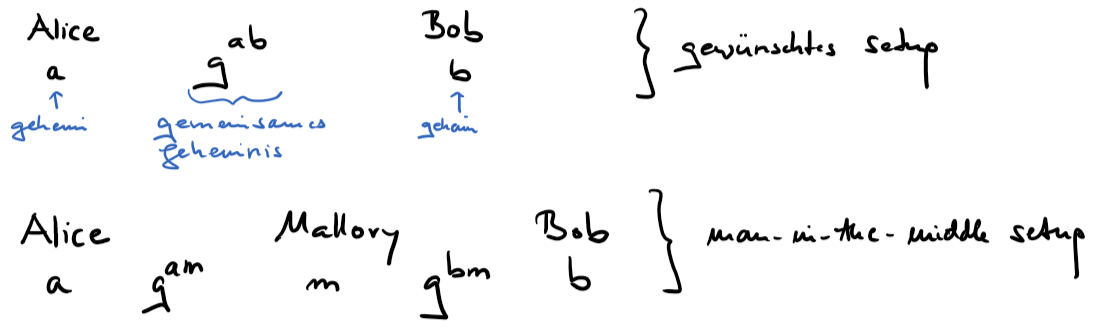
\includegraphics[width=12cm]{bild3.png}

Mallory kontrolliert das Netzwerk. Er gibt sich gegenüber Alice als Bob aus und gegenüber Bob als Alice. Mit beiden vereinbart er getrennte Schlüssel $g^{am}$ und $g^{bm}$.
\end{frame}


 %---
\begin{frame}[fragile]

\textbf{RSA-Verfahren} \pause

Alice wählt zwei Primzahlen $p$ und $q$ und berechnet $m = p \cdot q$ und $\tilde{m} = (p-1)(q-1)$. \pause
Alice wählt Verschlüsselungsexponent $e$ mit $1 < e < \tilde{m}$ und $\ggT(e,\tilde{m}) = 1$ \pause und berechnet Entschlüsselungsexponent $d$ mit $\overline{d} = \dfrac{\overline{1}}{\overline{e}}$ in $\mathbb{Z}_{\tilde{m}}$. \pause

Dann ist der öffentliche Schlüssel  $(m,e)$ und der private Schlüssel $(m,d)$. \pause

Für die zu verschlüsselnde Nachricht muss gelten: $0<n<m$. \pause

Bob verschlüsselt $n: \quad N = n^e \tmod m$ \\ \pause
Alice entschlüsselt $N: \quad n = N^d \tmod m$ 
\end{frame}


 %---
\begin{frame}[fragile]
Beispiel: $p = 7, q = 13 \pause \Rightarrow m = 91$ (RSA-Modul), $\tilde{m} =  72$ \pause
$e =11, \pause \ggT(e,\tilde{m}) = 1$. \\ \pause
Berechnung von $d$:  $\overline{d} = \dfrac{\overline{1}}{\overline{e}}$ in $\mathbb{Z}_{\tilde{m}}$\pause, d.h. 
$\Mod{d \cdot e}{1}{\tilde{m}}$\pause, also $d \cdot e - 1 = k \cdot \tilde{m}$ für ein  $k \in \mathbb{Z}$. \\ \pause
Wir lösen die diophantische Gleichung $d \cdot 11 - k \cdot 72 = 1$ \pause mit dem Erweiterten Euklidschen Algorithmus und erhalten $d=59$. \pause Der öffentliche Schlüssel ist $(91,11)$, der private Schlüssel ist $(91,59)$. \pause

Bob verschlüsselt $n=10: \pause \quad N= 10^{11} \tmod 91 = 82$  \\ \pause
Alice entschlüsselt $N=82: \pause \quad n = 82^{59} \tmod 91 = 10$ \pause

\footnotesize
\begin{tabular}{l l}
Nebenrechnungen (mod 91)  &    $82^1 \equiv -9 $ \\
$10^1 \equiv 10 $ & $82^2 \equiv 81 \equiv -10$\\
$10^2 \equiv 9 $ & $82^4 \equiv 9$\\
$10^4 \equiv -10 $ & $82^8 \equiv -10$\\
$10^8 \equiv 100 \equiv 9$ & $82^{16} \equiv 9$\\
$10^{11} \equiv 9 \cdot 9 \cdot 10 \equiv -100 \equiv 82$ & $82^{32} \equiv -10$\\
&  $82^{59} \equiv 82^{32+16+8+2+1} \equiv -10 \cdot 9 \cdot -10 \cdot -10 \cdot -9 \equiv 10$
\end{tabular}
\end{frame}

 %---
\begin{frame}[fragile]

\textbf{Beweis, dass RSA-Entschlüsselung funktioniert} \pause

Wir zeigen $n = N^d \tmod m$, indem wir zeigen: $(n^e)^d \equiv n \tmod m$. \pause Wir zeigen
zunächst: \\
$(1): (n^e)^d \equiv n \tmod p \quad  $ und $(2): (n^e)^d \equiv n \tmod q \quad (2)$  \pause

Es ist $\overline{d} = \dfrac{\overline{1}}{\overline{e}}$ in $\mathbb{Z}_{\tilde{m}}$\pause, also gilt: $de - 1 = k \tilde{m}$. \pause Daraus folgt: $de = 1 + k\tilde{m} = 1+k(p-1)(q-1)$. \pause Beweis von (1):  \\ \pause
Fall 1: $p|n \pause \Rightarrow n \equiv 0 \tmod p \pause \Rightarrow (n^e)^d \equiv 0 \tmod p$. \\ \pause
Fall 2: $p \nmid n$ \pause $\Rightarrow (n^e) ^d = n^{ed} = n^{1+k(p-1)(q-1)}\pause = n \cdot (n^{p-1})^{k(q-1)} \pause \equiv n \tmod p$\pause, 
da $n^{p-1}\equiv 1 \tmod p$ nach dem kleinen Satz von Fermat. \pause \\ Beweis von (2) analog. \\ \pause
Aus (1) und (2) folgt: $(n^e)^d - n = k_1 \cdot p = k_2 \cdot q$. mit geeigneten $k_1, k_2 \in \mathbb{Z}$. \pause Da $p, q$ Primzahlen, steckt $k_1$ in $q$ und $k_2$ in $p$. \pause
Also gilt:  $(n^e)^d - n = k_3 \cdot p \cdot q$. \pause Daraus folgt  $(n^e)^d \equiv n \tmod m. \hfill \square{}$

\end{frame}

 %---
\begin{frame}[fragile]

\textbf{Angriff auf das RSA-Verfahren} \pause

Die Sicherheit des Verfahrens hängt davon ab, dass der Angreifer das öffentlich bekannte $m$ nicht in die beiden
Primfaktoren $p$ und $q$ zerlegen kann. \pause Sonst könnte er $\tilde{m}$ berechnen und dann auch das Inverse zu dem öffentlichen $e$ in $\mathbb{Z}_{\tilde{m}}$. 
\end{frame}

 %---
\begin{frame}[fragile]

\textbf{Aufwand für die Faktorensuche} \pause

Wenn wir versuchen, die Faktoren einer Primzahl mit 300 Stellen zu finden, testen wir nur Primzahlen, die kleiner als
$\sqrt{10^{300}} = 10^{150}$ sind. \pause Nach der Abschätzung von Euler gilt für große $n$, dass es ca. $\frac{n}{\ln(n)}$ Primzahlen unterhalb von $n$ gibt. \\ \pause
$\ln(10^{150}) \pause = 150 \cdot \ln(10) \approx 150 \cdot 2.3 = 345.4$. \pause Also müssen wir $\frac{10^{150}}{345.5} \approx 3 \cdot 10^{147}$ Kandidaten testen. \pause

Annahme: 1 Computer schaft $10^{12}$ Prüfungen pro Sekunde (1 Million Millionen). \pause Das sind im Dauerbetrieb pro Jahr: 
$10^{12} \cdot 60 \cdot 60 \cdot 24 \cdot 365 \approx 3 \cdot 10^{19}$ Prüfungen. \pause Das bedeutet  
$\frac{3 \cdot 10^{147}}{3 \cdot 10^{19}} = 10^{128}$ Jahre für alle Prüfungen (Alter des Weltalls: ca. $10^{10}$ Jahre). \pause

Wenn jeder Mensch einen Computer beisteuern würde und manche zwei kämen wir auf 10 Millarden = $10^{10}$ Computer. \pause Wenn jeder dieser Computer 1000 mal schneller wäre, würde es immer noch $10^{128-10-3} = 10^{115}$ Jahre dauern.
\end{frame}

%---
\begin{frame}[fragile]

\textbf{Kryptographische Hashfunktionen} \pause

Hashfunktionen bilden Eingabewerte (z.B. ein Text oder eine Datei) auf einen Wert fester Länge ab, den \textit{Hash} der Eingabe. \pause Beispiel: \textit{SHA-256} bildet Eingaben auf eine Bitfolge der Länge 256 ab. \pause

Kryptographische Hashfunktionen sind kollisionsresistene Einwegfunktionen. \pause Kollisionsresistent bedeutet, es ist praktisch unmöglich, zwei Eingaben zu finden, die denselben Hash ergeben. \pause Einwegfunktion bedeutet, es ist praktisch unmöglich, aus dem Hashwert den Eingabewert zu rekonstruieren.

\end{frame}

%---
\begin{frame}[fragile]

\textbf{Digitale Signatur}

Mit dem RSA-Verfahren und einer kryptographischen Hashfunktion kann eine digitale Signatur erstellt werden. \pause

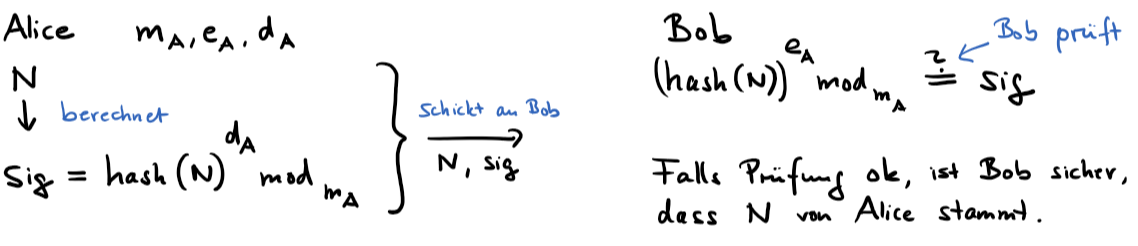
\includegraphics[width=12cm]{bild4.png}
\end{frame}


%---
\begin{frame}[fragile]

Durch eine digitale Signatur wird der Diffie-Hellman Schlüsselaustausch vor einem
Man-in-the-middle-Angriff geschützt. \pause

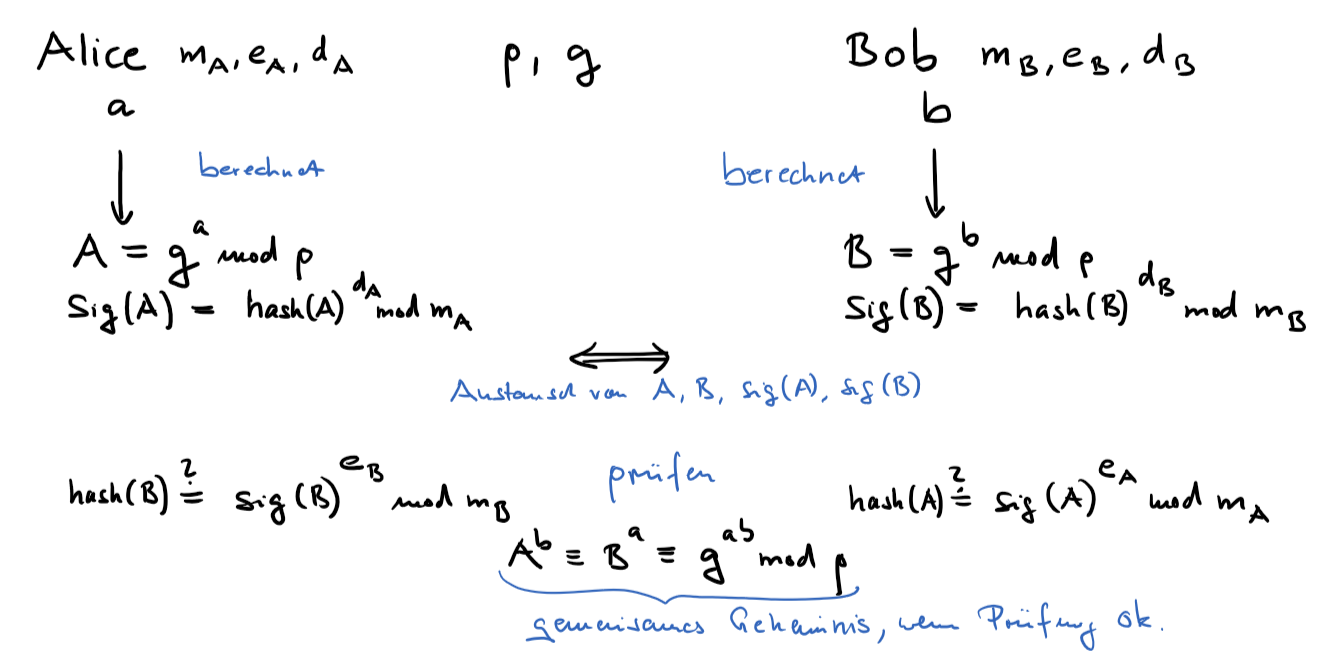
\includegraphics[width=12cm]{bild5.png}
\end{frame}


\end{document}